\documentclass[12pt]{article}
\usepackage[letterpaper,margin=1in]{geometry}
\usepackage[T1]{fontenc}
\usepackage[utf8]{inputenc}
\usepackage{lmodern}
\usepackage{amsmath,amssymb,amsthm}
\usepackage{graphicx,booktabs,array,multirow,caption,microtype}
\graphicspath{{docs/report/figures/}{figures/}}
\usepackage{enumitem,tikz,xcolor,float,titlesec}
\usepackage{subcaption}
\DeclareCaptionLabelFormat{actionpanel}{Figure~\thefigure#2}
\usetikzlibrary{arrows.meta,positioning,fit,backgrounds}
\usepackage[hidelinks]{hyperref}
\captionsetup{font=footnotesize,skip=3pt}
\providecommand{\tightlist}{\setlength{\itemsep}{0pt}\setlength{\parskip}{0pt}}
\setlength{\parindent}{1.2em}
\setlength{\parskip}{0pt}
\widowpenalty=10000
\clubpenalty=10000
\setlength{\textfloatsep}{7pt plus 2pt minus 2pt}
\setlength{\intextsep}{7pt plus 2pt minus 2pt}
\setlength{\abovedisplayskip}{5pt}
\setlength{\belowdisplayskip}{5pt}
\setlength{\abovedisplayshortskip}{3pt}
\setlength{\belowdisplayshortskip}{3pt}
\titlespacing*{\section}{0pt}{8pt}{3pt}
\titlespacing*{\subsection}{0pt}{6pt}{2pt}
\renewcommand{\arraystretch}{0.94}
\newcommand{\real}{\mathbb{R}}
\newcommand{\expect}{\mathbb{E}}
\newcommand{\indic}{\mathbb{I}}
\newcommand{\sg}{\operatorname{sg}}
\DeclareMathOperator*{\argmin}{arg\,min}
\DeclareMathOperator*{\argmax}{arg\,max}
\begin{document}
\begin{center}
{\LARGE\bfseries Imagine Before You Push\par}
\vspace{0.35em}
{\scriptsize Liu Ernest Hin Yui \quad Wong Deshun \quad Harsh Rao Dhanyamraju \quad Arnav Goel \quad Alez Ng Rui Jie \quad Maahir Garg\par}
\vspace{0.05em}
{\footnotesize School of Computing, National University of Singapore\par}
\end{center}
\vspace{-0.8em}

\begin{abstract}
We investigate whether an explicit physics simulator can serve as a reinforcement-learning
agent's imagination to improve control under unseen or out-of-distribution (OOD) dynamics.
As a proxy task, we study toppling-safe pushing: moving an upright cuboid to a goal without
knocking it over, a problem relevant to handling fragile items in warehouses. The object's
mass $m$, floor friction coefficient $\mu$, and centre-of-mass (COM) height $h_c$ are hidden.
The agent observes only the remaining goal distance $d$, tilt $\psi$, translational velocity
$\dot{x}$, angular velocity $\dot{\psi}$, and geometry $G$, making the task partially
observable. Our approach combines online Bayesian system identification using Sequential
Monte Carlo squared (SMC\textsuperscript{2}) to infer the hidden parameters, a physics
engine to forecast candidate actions, and a customised soft actor--critic (SAC) policy called
the delta actor--critic to select pushes. Direct training collapses to an inactive policy,
while a reverse curriculum yields approximately 81\% success across 1.0\,m training episodes.
At 1.0\,m, physics has lower recorded toppling than both comparators.
Held-out OOD success is 47.5\% for physics, 33.8\% for the learned model,
and 3.8\% for model-free control. These
results support our hypothesis that explicit tipping mechanics provide useful structure
for imagination under unfamiliar dynamics. Although the study is exploratory and entirely
sim-to-sim, system-identification analysis also shows that successful control can persist
despite substantial parameter-estimation errors, with some OOD shifts remaining challenging.
\end{abstract}

\section{Introduction}\label{sec:intro}
Reinforcement learning under unfamiliar dynamics requires forward models that remain useful beyond training. Learned world models predict action outcomes from experience, while explicit simulators encode rigid-body mechanics and can be reconfigured for new objects. This physical structure may support generalisation to unseen objects if the agent can infer the relevant hidden parameters. We investigate whether a physics simulator with online SysID supports more reliable control than a learned neural world model.

We use \emph{toppling-safe pushing as a proxy task}: moving an upright cuboid to a goal without toppling it. Identical geometries can conceal different masses, friction coefficients, and COM heights. Small tilt-prediction errors can cause task-ending failures, making pushing an informative test of forecasts used for safe decisions.

We compare an explicit PyBullet forward model configured through Bayesian system identification (SMC\textsuperscript{2}), a learned neural world model, and a model-free baseline with no imagined trajectories. Both forward models use the customised delta actor--critic framework. We ask whether \textbf{physics-based imagination, adapted online through SysID, provides more reliable control under unseen dynamics than learned imagination or no forward model}.

All experiments are sim-to-sim: independent target and internal environments share PyBullet mechanics. They test generalisation under parameter shifts; arbitrary simulator mismatch and real-world transfer remain untested.

Our contributions are:
\begin{enumerate}[leftmargin=1.6em,itemsep=1pt,topsep=2pt,beginpenalty=10000]
\item A physics-based forward-model pipeline that infers hidden parameters with
SMC\textsuperscript{2} and uses simulated trajectories in a customised delta actor--critic.
\item A comparison of three methods during curriculum training and held-out OOD evaluation.
\item An analysis of imperfect SysID and control, examining parameter errors and the object's tip-stability margin.
\item A reverse curriculum that overcomes policy inaction and makes the forward-model
comparison possible at longer target distances.
\end{enumerate}

\section{Related Work}\label{sec:related}
Model-based RL uses predicted outcomes to improve decisions. Dyna-style methods combine real and simulated experience \cite{sutton1990}; MBPO learns a dynamics model, although prediction errors can bias the resulting policy \cite{mbpo}. Our study compares how explicit and learned forecasts support control near tipping.

When object dynamics are unknown, the forward model must adapt. SimOpt and BayesSim infer simulator parameters from observations \cite{simopt,bayessim}, while UPOSI and RMA use histories of past interactions \cite{uposi,rma}. We instead retain a particle posterior over plausible physical parameters and score actions across that distribution.

Our approach also differs from hard safety shielding \cite{shield} and constrained pushing \cite{dadiotis}. Safety enters through the critic's predicted values, not a formal action constraint. For training, we build on reverse curriculum learning \cite{florensa2017}, gradually increasing the target distance as the policy improves.

\section{Problem Formulation}\label{sec:formulation}
\subsection{Object, observation, and action}\label{sec:objects}
The cuboid's observable geometry is $G=(w,\ell,H)$, with width $w$ along the pushing direction, depth $\ell$, and height $H$. Its hidden parameters are $\theta=(m,\mu,h_c)$: mass, floor friction, and COM height. We infer them in normalised coordinates $z=(\log m,\mu,h_c/H)$ under a bounded prior. The policy observes
\begin{equation}o_t=(d_t,\psi_t,\dot x_t,\dot\psi_t,w,\ell,H)\in\real^7,\label{eq:obs}\end{equation}
where $d_t$ is signed distance to the goal, $\psi_t$ is tilt, and the two velocities $\dot x_t$ and $\dot\psi_t$ capture ongoing motion. Hidden dynamics make the task a POMDP. The true $\theta$ is stored for evaluation but is not revealed to the controller.

Each push applies an action $a_t=(h_t,F_t,\tau_t)$ at time $t$, with contact height $h_t\in[0.1H,0.9H]$, forward force $F_t\in[0,F_{\max}]$, and duration $\tau_t\in[0.05,0.50]$\,s. The action is normalised to $[-1,1]^3$. Translation is one-dimensional, but the cuboid can rotate and topple. Episodes end on success, toppling, or a timeout (i.e. reached a maximum number of actions per episode, $T_{\max}$).

\begin{figure}[htbp]
\centering
\captionsetup[subfigure]{labelformat=actionpanel,labelsep=colon,font=footnotesize}
\begin{subfigure}[b]{0.53\textwidth}
\centering
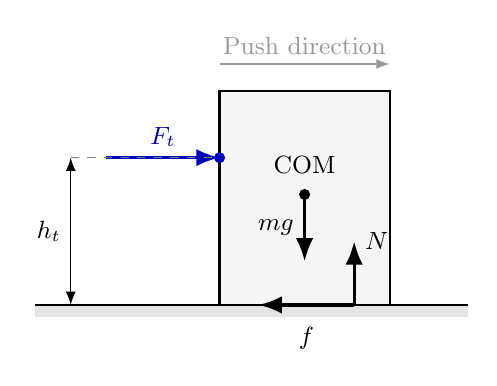
\begin{tikzpicture}[>=Latex, x=0.9cm, y=0.85cm,
    force/.style={->,very thick}, dimension/.style={<->,thin},
    every node/.style={font=\small}]
\fill[gray!8] (0,0) rectangle (2.4,3.2);
\draw[thick] (0,0) rectangle (2.4,3.2);
\fill[gray!20] (-2.6,-0.18) rectangle (3.5,0);
\draw[thick] (-2.6,0) -- (3.5,0);
\draw[force,blue!75!black] (-1.6,2.2) -- (0,2.2)
    node[midway,above] {$F_t$};
\fill[blue!75!black] (0,2.2) circle (2pt);
\draw[gray,dashed] (-2.1,2.2) -- (-0.1,2.2);
\draw[dimension] (-2.1,0) -- (-2.1,2.2) node[midway,left] {$h_t$};
\fill (1.2,1.65) circle (2pt);
\node[above=4pt] at (1.2,1.65) {COM};
\draw[force] (1.2,1.65) -- (1.2,0.65) node[midway,left] {$mg$};
\draw[force] (1.9,0) -- (1.9,0.95) node[right] {$N$};
\draw[force] (1.9,0) -- (0.55,0) node[midway,below=4pt] {$f$};
\draw[->,gray!80] (0,3.6) -- (2.4,3.6)
    node[midway,above] {Push direction};
\end{tikzpicture}
\caption{Forces and contact height.}\label{fig:push-forces}
\end{subfigure}\hfill
\begin{subfigure}[b]{0.43\textwidth}
\centering
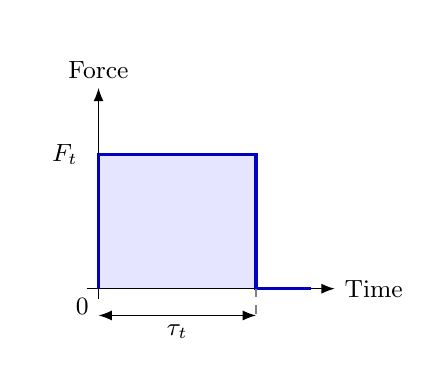
\begin{tikzpicture}[>=Latex,x=1cm,y=0.85cm,
    every node/.style={font=\small}]
\path[use as bounding box] (-0.9,-0.85) rectangle (3.8,3.9);
\fill[blue!10] (0,0) rectangle (2.0,2.0);
\draw[->] (-0.15,0) -- (3.0,0) node[right] {Time};
\draw[->] (0,-0.15) -- (0,3.0) node[above] {Force};
\draw[very thick,blue!75!black]
    (0,0) -- (0,2.0) -- (2.0,2.0) -- (2.0,0) -- (2.7,0);
\node[left=4pt] at (0,2.0) {$F_t$};
\node[below left] at (0,0) {$0$};
\draw[dashed,gray] (2.0,0) -- (2.0,-0.45);
\draw[<->,thin] (0,-0.4) -- (2.0,-0.4)
    node[midway,below] {$\tau_t$};
\end{tikzpicture}
\caption{Force and duration.}\label{fig:push-duration}
\end{subfigure}
\caption{Push action $a_t=(h_t,F_t,\tau_t)$. A horizontal force $F_t$ is applied at height $h_t$ above the floor for duration $\tau_t$. Weight $mg$, normal reaction $N$, and floor friction $f$ are shown schematically.}
\label{fig:push-action}
\end{figure}


\subsection{Tipping and the stability margin}\label{sec:topple}
The simplified rigid-body stability condition for sliding without tipping is as follows,
\begin{equation}\frac{F}{mg}(h-h_c)\leq\underbrace{\frac{w}{2}-\mu h_c}_{\mathcal M(w,\mu,h_c)},\label{eq:topple}\end{equation}
where $\mathcal M$ is the \emph{tip-stability margin} \cite{hibbeler2022}. This relation is used to interpret results, not supplied to the agent. The margin depends on width, friction, and COM height but not mass. The left-hand side also depends on mass and COM height, so margin error alone cannot establish an accurate tipping prediction.

Toppling is recorded at push end if $|\psi|>\arctan(w/(2h_c))$, when the COM projection passes the supporting edge (Appendix~\ref{app:toppling-threshold}). This endpoint criterion differs from the force-based condition and does not measure intermediate threshold crossings.

\subsection{Reward Function}\label{sec:reward}
The reward function favours \textbf{progress}, \textbf{settling at the goal}, and \textbf{avoiding toppling}. We use the potential $\phi(d)=-A|d|+B\kappa/(|d|+\kappa)$, where $A$ controls the distance term, $B$ bounds the closeness bonus, and $\kappa$ sets its distance scale. The per-decision reward is
\begin{equation}\begin{aligned}
r_t={}&\underbrace{\phi(d_t)-\phi(d_{t-1})}_{\text{progress shaping}}-P_{\mathrm{np}}\indic_t^{\mathrm{np}} -c_{\mathrm{time}}\tau_t-c_{\mathrm{step}}+R_{\mathrm{succ}}\indic_t^{\mathrm{succ}}-R_{\mathrm{topple}}\indic_t^{\mathrm{topple}}.
\end{aligned}\label{eq:reward}\end{equation}
\textbf{Progress shaping} ($\phi(d_t)-\phi(d_{t-1})$) rewards movement toward the goal and penalises overshooting through $|d|$. This undiscounted potential difference carries no policy-invariance guarantee for $\gamma=0.99$. The \textbf{no-progress penalty} ($-P_{\mathrm{np}}\indic_t^{\mathrm{np}}$) discourages inactivity. \textbf{Time and step costs} ($-c_{\mathrm{time}}\tau_t-c_{\mathrm{step}}$) favour efficient pushes; \textbf{terminal rewards} ($+R_{\mathrm{succ}}\indic_t^{\mathrm{succ}}-R_{\mathrm{topple}}\indic_t^{\mathrm{topple}}$) distinguish success from toppling. Success requires settling within position and tilt tolerances at low speed. For the proposed method, an \textbf{optional uncertainty-reduction bonus} ($\beta\max(0,V_{t-1}-V_t)$) rewards decreases in posterior spread. Here $V_t$ sums the posterior-weighted variances of the $z$ coordinates, each scaled to its prior range. This is a heuristic, not a measure of Bayesian information gain. Full settings are in Appendix~\ref{app:hp}.

\section{Method}\label{sec:method}
\subsection{Architecture and simulator}\label{sec:arch}


\begin{figure}[htbp]
\centering
\resizebox{\textwidth}{!}{%
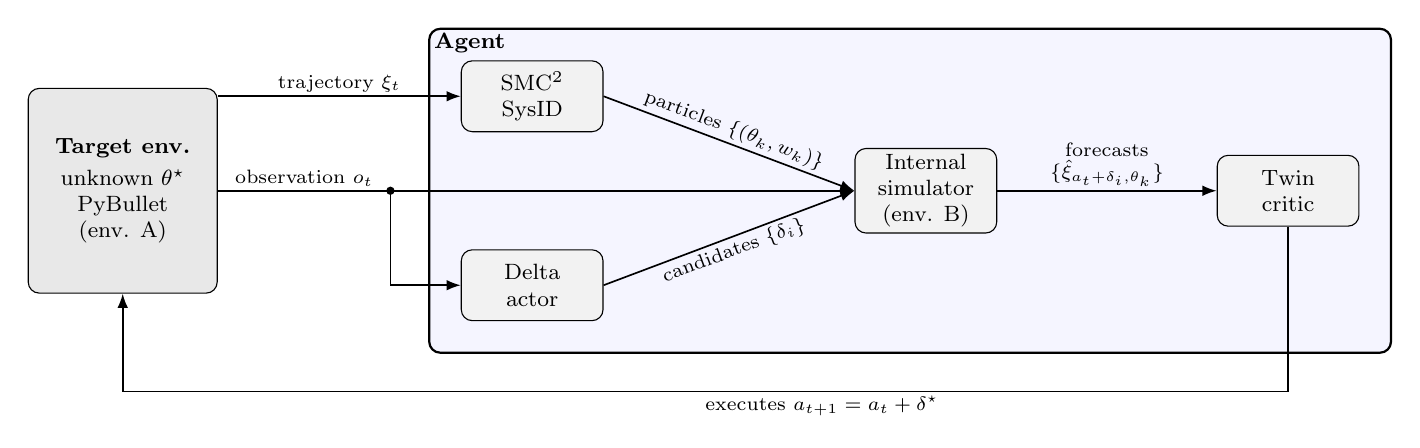
\begin{tikzpicture}[
font=\footnotesize, >={Latex[length=1.8mm]},
comp/.style={draw,rounded corners,fill=gray!10,align=center,minimum width=18mm,minimum height=9mm,inner sep=2pt},
env/.style={draw,rounded corners,fill=gray!18,align=center,minimum width=24mm,minimum height=26mm},
lab/.style={font=\scriptsize,inner sep=1.3pt},
flow/.style={->,semithick}]
\node[env] (env) at (-5.2,0) {\textbf{Target env.}\\[2pt]unknown $\theta^\star$\\PyBullet\\(env. A)};
\node[comp] (sysid) at (0,1.2) {SMC\textsuperscript{2}\\SysID};
\node[comp] (actor) at (0,-1.2) {Delta\\actor};
\node[comp] (sim) at (5.0,0) {Internal\\simulator\\(env. B)};
\node[comp] (critic) at (9.6,0) {Twin\\critic};
\begin{scope}[on background layer]
\node[draw,thick,rounded corners,fill=blue!4,inner sep=4mm,fit=(sysid)(actor)(sim)(critic)] (agent) {};
\end{scope}
\node[anchor=north west,font=\footnotesize\bfseries,inner sep=2pt] at (agent.north west) {Agent};
\draw[flow] (env.east|-sysid) -- node[lab,above]{trajectory $\xi_t$} (sysid.west);
\coordinate (obs) at (-1.8,0);
\draw[semithick] (env.east) -- node[lab,above]{observation $o_t$} (obs);
\fill (obs) circle (1.5pt);
\draw[flow] (obs) |- (actor.west);
\draw[flow] (obs) -- (sim.west);
\draw[flow] (sysid.east) -- node[lab,above,sloped,pos=0.5]{particles $\{(\theta_k,w_k)\}$} (sim.west);
\draw[flow] (actor.east) -- node[lab,below,sloped,pos=0.5]{candidates $\{\delta_i\}$} (sim.west);
\draw[flow] (sim.east) -- node[lab,above,align=center]{forecasts\\$\{\hat{\xi}_{a_t+\delta_i,\theta_k}\}$} (critic.west);
\coordinate (ret) at (9.6,-2.55);
\draw[flow] (critic.south) -- (ret) -| node[lab,pos=0.2,below]{executes $a_{t+1}=a_t+\delta^\star$} (env.south);
\end{tikzpicture}%
}
\caption{Simplified data flow between independent target and internal PyBullet environments. SMC\textsuperscript{2} infers physics hypotheses from observed motion; the simulator forecasts candidate pushes; the twin critic ranks them.}\label{fig:arch}
\end{figure}

The target PyBullet environment \cite{pybullet} provides observation $o_t$ to the delta actor, which proposes corrections $\{\delta_i\}$ to the last executed action $a_t$, giving candidates $a_{t+1}^{(i)}=a_t+\delta_i$. After execution of an action, the environment records a trajectory $\xi_t$ for SMC\textsuperscript{2}. The estimator updates hypotheses $\{(\theta_k,w_k)\}$, where $\theta_k$ contains candidate physical parameters and $w_k$ is its posterior weight, calculated in Section~\ref{sec:sysid}. A separate headless PyBullet simulator reconstructs the cuboid's pose and velocities from $o_t$ and forecasts $\hat{\xi}_{a_t+\delta_i,\theta_k}$ for each candidate under each hypothesis. The twin critics score each candidate using these forecasts; the highest-scoring correction $\delta^\star$ determines the next executed action, $a_{t+1}=a_t+\delta^\star$ (Figure~\ref{fig:arch}).

Our focus on OOD generalisation motivates a key design choice: estimated physical parameters configure only the internal simulator, never the actor or critic inputs. \textbf{Appending OOD parameter estimates would introduce distributional drift into the networks' inputs}. The simulator instead translates those estimates into predicted motion. Scaling mass and force together can yield similar trajectories under comparable contact conditions. This motivates using trajectories, but does not guarantee familiar network inputs: unfamiliar physics can also produce unfamiliar motion.

\subsection{Online system identification (SMC\texorpdfstring{\textsuperscript{2}}{2})}\label{sec:sysid}
Our SMC\textsuperscript{2} estimator \cite{smc2} uses a bounded uniform prior in $z$, making mass log-uniform. Under $\theta_k$, one replay of push $a_t$ from measured state $s_t$ predicts $\hat{\xi}_{t;\,a_t,\theta_k}(s_t)$. This reduces inference to SMC over physical parameters, with resampling and Metropolis--Hastings rejuvenation. We compare the forecast with recorded $\xi_t$, modelling channel $c\in\{x,\psi,\dot x,\dot\psi\}$ at sampled timestep $n$ as

\begin{equation}\label{eq:sample-likelihood}
\xi_{t,n}^{c}\mid\theta_k,s_t
\sim\mathcal N\!\left(
[\hat{\xi}_{t;\,a_t,\theta_k}(s_t)]^c_n,\sigma_c^2
\right).
\end{equation}
Assuming independent residuals across channels and sampled timesteps, the trajectory log-likelihood is equivalently given by
\begin{equation}\label{eq:trajectory-likelihood}
\log p(\xi_t\mid \theta_k,s_t)=-\frac12\sum_c\sum_{n=1}^{N_t}\left[
\frac{(\xi^c_{t,n}-[\hat{\xi}_{t;\,a_t,\theta_k}(s_t)]^c_n)^2}{\sigma_c^2}+\log(2\pi\sigma_c^2)\right].
\end{equation}
Here $\sigma_c$ is a fixed likelihood hyperparameter (Appendix~\ref{app:likelihood-calibration}) controlling the tolerated prediction error in channel $c$. We evaluate the likelihood using $N_t$ trajectory samples selected at a fixed sampling stride.

Sequential importance sampling updates the $N_\theta$ parameter-particle weights using the likelihood of each new trajectory, with $\sum_{k=1}^{N_\theta}w_{t,k}=1$:
\begin{equation}
w_{t,k}=\frac{w_{t-1,k}p(\xi_t\mid \theta_k,s_t)}
{\sum_j w_{t-1,j}p(\xi_t\mid \theta_j,s_t)}.
\label{eq:weightupdate}\end{equation}
Over time, a few hypotheses can dominate these weights. We measure this weight degeneracy using the effective sample size (ESS) \cite{smc2}:
\begin{equation*}\mathrm{ESS}=\left(\sum_{k=1}^{N_\theta}(w_{t,k})^2\right)^{-1}.\end{equation*}
When ESS falls below a configured fraction of $N_\theta$, systematic resampling favours high-weight particles but can create duplicates. Metropolis-Hastings MCMC moves \cite{hastings1970} then restore diversity. The random-walk proposal covariance adapts to the weighted particle cloud. In the transformed coordinates from Section~\ref{sec:objects}, a symmetric proposal from $z$ to $z'$ is accepted with probability
\begin{equation}\label{eq:mh-accept}
\alpha_{\mathrm{MH}}(z\to z')=\min\left\{1,\frac{p(z')\prod_{i=1}^{t}p(\xi_i\mid z')}{p(z)\prod_{i=1}^{t}p(\xi_i\mid z)}\right\}.
\end{equation}
The prior ratio is one for two in-prior hypotheses. The reported configuration uses $N_\theta=32$ outer particles and two MCMC moves per resampling event. The controller forecasts actions under the full particle population, including any duplicates. For critic evaluation, we write $K=N_\theta$ and $w_k=w_{t,k}$, with $\sum_{k=1}^{K}w_k=1$.

\subsection{Delta actor--critic}\label{sec:delta}
\textbf{A policy that predicts action $a_t$ directly, rather than a correction $\delta_i$, may struggle with OOD objects that require forces outside the range of actions output during training.} Building on SAC \cite{sac,sacauto}, our actor samples bounded corrections relative to a reference action $a_{\mathrm{ref}}$, which is the last executed action $a_t$ under the convention in Section~\ref{sec:arch}. Each episode begins with a predefined probe $a_0$, after which $a_{\mathrm{ref}}=a_0$. At each decision, candidate actions are formed as $a_{\mathrm{ref}}+\delta_i$. Once the selected action is executed, it becomes the reference for the next decision: $a_{\mathrm{ref}}\leftarrow a_{\mathrm{ref}}+\delta^\star$.

These successive corrections let the controller adjust the pushing force gradually rather than extrapolating to a large absolute action.

\textbf{Bounded action sampling.} The actor predicts a Gaussian mean $\mu_\phi$ and standard deviation $\sigma_\phi$. Bounds $[l,u]$ limit the correction while keeping $a_{\mathrm{ref}}+\delta$ within $[-1,1]^3$. Following the reparameterisation trick \cite{kingma2013}, we transform standard Gaussian noise $\mathbf e$, apply $\tanh$, and rescale to $[l,u]$ to keep corrections $\delta$ feasible:
\begin{equation}\label{eq:squash}
\mathbf e\sim\mathcal N(0,I),\quad \rho=\mu_\phi+\sigma_\phi\odot\mathbf e,\quad
\delta=\frac{u+l}{2}+\frac{u-l}{2}\odot\tanh(\rho).
\end{equation}

\subsubsection{Trajectory encoder}
Both the actor and twin critics use a shared attention-based encoder $e(\cdot)$ to convert recorded and simulated trajectories into feature vectors. It adapts the Transformer architecture \cite{transformer} to variable-length pushing trajectories, using a learned CLS token to summarise each sequence and padding masks to exclude unused timesteps. The critic optimiser trains the shared encoder, while the actor optimiser updates only the policy head.

For correction $\delta$, the simulator forecasts $\hat{\xi}_{a_{\mathrm{ref}}+\delta,\theta_k}$. The controller context $c$ contains observation $o$, latest recorded trajectory $\xi^{\mathrm{real}}$ (the context-specific $o_t$ and $\xi_t$), reference action $a_{\mathrm{ref}}$, and posterior hypotheses. The controller uses $a_{\mathrm{ref}}$ to bound corrections and construct candidate pushes, but does not append it to actor or critic network inputs. This design aims to reduce distributional drift from unfamiliar absolute action values. The two critic heads have network parameters $\omega_1,\omega_2$, distinct from physical parameters $\theta_k$. The critic averages forecast values across hypotheses, then takes the minimum across heads:
\begin{equation}
Q(c,\delta)=\min_{j\in\{1,2\}}\sum_{k=1}^{K}w_k
Q_{\omega_j}\!\left(o,e(\xi^{\mathrm{real}}),\delta,e(\hat{\xi}_{a_{\mathrm{ref}}+\delta,\theta_k})\right).
\label{eq:critic}\end{equation}
Learned values can penalise predicted toppling, but posterior-weighted ranking imposes no safety constraint across all hypotheses.

\textbf{Learning with a non-differentiable simulator.} PyBullet does not expose gradients through imagined trajectories. Differentiating only through the critic's explicit action input would ignore how the forecast changes with the action and could give a wrong gradient. We therefore use a likelihood-ratio (score-function) estimator \cite{reinforce} for the critic-value term, with the stored replay action as a variance-reducing baseline:
\begin{equation}\begin{aligned}
\mathcal L_\pi=\expect\!\Big[&\alpha\log\pi_{\mathrm{path}}(\delta\mid c)-\sg\!\big(Q(c,\delta)-Q(c,\delta^{\mathrm{replay}})\big)\log\pi_{\mathrm{sc}}(\delta)\Big].
\end{aligned}\label{eq:actor}\end{equation}
The stored replay correction $\delta^{\mathrm{replay}}$ is fixed independently of the newly sampled correction $\delta$; its critic value serves as a variance-reducing baseline. Here $\sg$ stops gradients through the value term; $\pi_{\mathrm{sc}}$ evaluates the log-density at a fixed sampled action, and $\pi_{\mathrm{path}}$ retains the differentiable sampling path for the entropy term. The critics learn from one-step soft TD targets: the observed reward plus a discounted estimate of the next action's value, including SAC's entropy term. Terminal outcomes do not bootstrap, while time-limit truncations can. The full soft TD target and entropy-temperature update are in Appendix~\ref{app:actor-details}.

\subsection{Candidate selection}\label{sec:candidates}
The actor proposes a batch of feasible deltas. For each one, the internal simulator predicts a trajectory under every physics hypothesis, and the twin critics select the highest-scoring candidate. During warm-up, uniform feasible deltas collect initial experience. Executed actions are chosen by ranking, whereas continuation actions in the TD target are sampled from the actor; the latter distinction matters for the learning objective.

\subsection{Learned-model and model-free comparators}\label{sec:comparators}
The learned-model variant replaces physics simulation and SysID with an MLP that predicts the next trajectory from the current observation, reference action, candidate correction, and latest recorded trajectory. It is trained online by minimising the mean squared error between its prediction for an executed action and the resulting observed trajectory. Its forecasts are passed to the delta actor--critic for candidate scoring (Appendix~\ref{app:learned-model}).

The model-free variant retains the delta actor--critic framework but replaces forecast inputs with zeros. It selects actions using the observation and recorded trajectory, without predicting future motion. Neither comparator uses physics SysID.

\section{Training: Reverse Curriculum}\label{sec:curriculum}
\subsection{A policy too timid to act}\label{sec:timid}
\emph{Direct training} at 0.25\,m produced only 0--5\% success. Costly toppling and rare successes made weak pushes attractive to the critic, and the actor gradually reduced force to zero.

\emph{Proximity-based reward shaping} and a \emph{no-progress penalty} encouraged pushing but caused overshooting in up to 76\% of episodes. We considered \emph{supervised critic pre-training} but did not run it because collected transitions contained too few successes. Instead, a \textbf{reverse curriculum} trained on shorter targets before increasing distance, supplying successful examples missing from direct training.

\subsection{Curriculum and decision horizon}
Each stage continues from the previous stage's network weights. The curriculum uses \textbf{13 target distances}, from 0.10\,m to 1.0\,m:
\begin{equation*}\begin{gathered}
D\in\{0.10,0.15,0.20,0.25,0.30,0.35,0.40,0.50,0.60,0.70,0.80,0.90,1.00\}\ \mathrm m.
\end{gathered}\end{equation*}

A safe policy often needs many small pushes. An earlier 20-decision limit caused every episode to time out by the 0.60\,m stage. Increasing the limit to 40 reduced horizon-limited episodes to about 6\% at 1.0\,m, with about 15 pushes per episode on average. Within some stages, overshoot initially rose before the policy learned to settle near the target. Appendix~\ref{app:extended-analysis} gives the detailed stage dynamics and horizon diagnostics.

\section{Experiments and Results}\label{sec:experiments}
\subsection{Setup}\label{sec:setup}
The physics run used 32 SMC\textsuperscript{2} particles and a self-attention encoder; both comparators used interpolation. All three used $F_{\max}=15$\,N, up to two batches of four candidates, $T_{\max}=40$, $\epsilon=0.08$\,m, and the same task reward; only physics received the posterior bonus ($\beta=50$, Section~\ref{sec:reward}). All completed training through 1.0\,m. Rates include early learning across 8,700 physics, 9,470 learned-model and 16,090 model-free episodes at the 13 reported distances.

Training objects were sampled uniformly over $m\in[0.5,1.5]$\,kg, $\mu\in[0.3,0.7]$, $h_c/H\in[0.35,0.60]$, $w,\ell\in[0.05,0.10]$\,m, and $H\in[0.12,0.25]$\,m. Small parameter regions containing the held-out in-distribution cases were excluded from sampling. The SysID prior was wider: $m\in[0.2,3.0]$\,kg, $\mu\in[0.1,1.1]$, and $h_c/H\in[0.20,0.80]$. Figure~\ref{fig:training-distribution} illustrates the training ranges and held-out regions.

\begin{figure}[htbp]
\centering
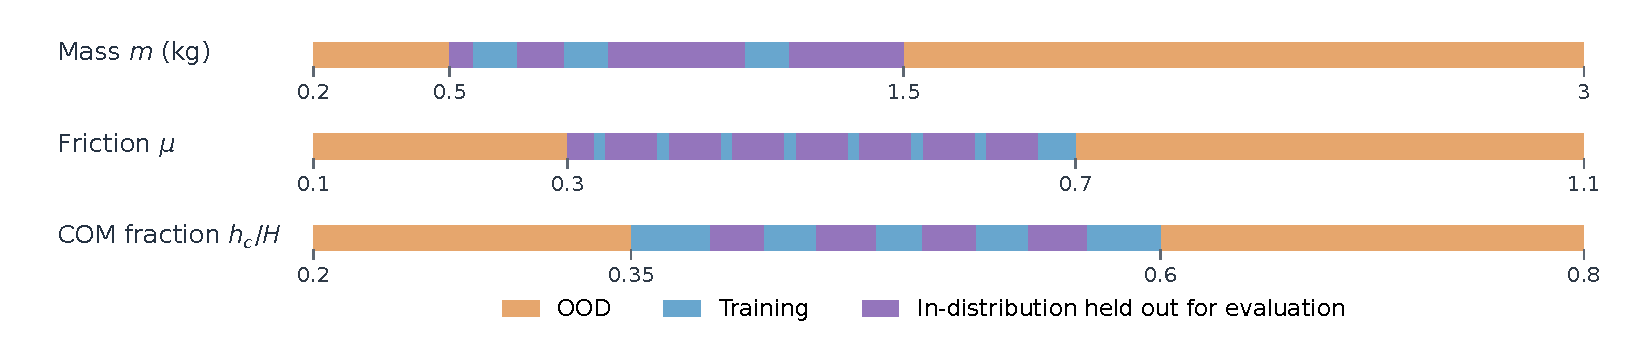
\includegraphics[width=\textwidth]{training_distribution_number_lines_draft.pdf}
\caption{Training and OOD parameter ranges. Purple intervals show projections of joint regions held out for in-distribution evaluation. Exclusion requires all three parameters to lie within one joint region.}
\label{fig:training-distribution}
\end{figure}

\subsection{Forward-model comparison and curriculum performance}\label{sec:reaching}
The physics curriculum reached 61.7\% success across the 0.25\,m stage and approximately 74\% over its final 25\% of training episodes. Success dipped to 62.4\% at 0.60\,m before recovering. Table~\ref{tab:curriculum} (Appendix~\ref{app:extended-analysis}) gives full stage outcomes, including early learning.

Table~\ref{tab:ablation} compares the three methods during training. At 1.0\,m, physics reached 80.6\% success with 13.6\% toppling, against 65.4\% and 26.3\% for the learned model, and 8.8\% and 87.7\% for model-free control. The learned model had higher success through 0.80\,m; physics led at 0.90 and 1.0\,m. Model-free control achieved occasional successes but remained unsafe.

\begin{table}[htbp]
\centering
\small
\setlength{\tabcolsep}{2pt}
\renewcommand{\arraystretch}{0.98}
\begin{tabular*}{\textwidth}{@{\extracolsep{\fill}}r *{12}{r}@{}}
\toprule
& \multicolumn{4}{c}{Physics (\%)} & \multicolumn{4}{c}{Learned (\%)} & \multicolumn{4}{c}{Model-free (\%)}\\
\cmidrule(lr){2-5}\cmidrule(lr){6-9}\cmidrule(lr){10-13}
Target (m) & S & T & TO & O & S & T & TO & O & S & T & TO & O\\
\midrule
0.10 & 31.1 & 32.6 & 27.9 & 8.4 & 43.7 & 40.0 & 4.2 & 12.1 & 2.1 & 84.0 & 12.4 & 1.4 \\
0.15 & 39.8 & 23.8 & 26.6 & 9.8 & 77.6 & 13.3 & 0.2 & 8.8 & 0.0 & 50.0 & 50.0 & 0.0 \\
0.20 & 65.4 & 23.2 & 1.3 & 10.1 & 74.8 & 17.7 & 0.0 & 7.4 & 3.6 & 89.0 & 5.0 & 2.3 \\
0.25 & 61.7 & 17.0 & 0.0 & 21.3 & 81.3 & 11.3 & 0.5 & 6.8 & 1.7 & 73.1 & 25.1 & 0.2 \\
0.30 & 78.3 & 9.2 & 1.5 & 10.9 & 88.2 & 7.4 & 0.7 & 3.8 & 0.6 & 99.0 & 0.2 & 0.2 \\
0.35 & 71.2 & 10.2 & 1.2 & 17.3 & 79.2 & 11.5 & 6.4 & 2.9 & 0.2 & 98.8 & 0.2 & 0.8 \\
0.40 & 74.7 & 10.2 & 6.5 & 8.6 & 80.0 & 11.6 & 2.2 & 6.2 & 1.6 & 97.4 & 0.0 & 1.0 \\
0.50 & 79.1 & 10.2 & 0.6 & 10.2 & 83.3 & 13.3 & 0.3 & 3.1 & 3.8 & 95.1 & 0.0 & 1.1 \\
0.60 & 62.4 & 12.9 & 12.5 & 12.2 & 80.0 & 16.9 & 0.3 & 2.8 & 3.3 & 94.2 & 0.0 & 2.5 \\
0.70 & 69.7 & 12.6 & 6.9 & 10.9 & 84.0 & 14.3 & 0.0 & 1.6 & 3.6 & 93.8 & 0.0 & 2.5 \\
0.80 & 77.3 & 16.4 & 2.2 & 4.2 & 81.6 & 16.9 & 0.0 & 1.5 & 4.0 & 92.2 & 0.0 & 3.8 \\
0.90 & 80.1 & 14.8 & 0.8 & 4.2 & 72.3 & 22.9 & 2.0 & 2.8 & 6.8 & 88.1 & 0.0 & 5.1 \\
1.00 & 80.6 & 13.6 & 1.7 & 4.1 & 65.4 & 26.3 & 2.4 & 6.0 & 8.8 & 87.7 & 0.0 & 3.5 \\
\bottomrule
\end{tabular*}
\caption{Curriculum outcome rates (\% of all episodes at each distance). S: success; T: topple, including toppled overshoots; TO: other timeout ($d\ge-0.08$\,m); O: overshoot timeout ($d<-0.08$\,m, beyond the goal tolerance).}
\label{tab:ablation}
\end{table}
The learned model's median trajectory MSE fell from 0.064 over the first 250 updates to 0.0032 over the last 250, yet 26.3\% of its 1.0\,m episodes toppled. Low aggregate prediction error alone did not guarantee safe control.

\subsection{System-identification accuracy and robustness}\label{sec:identifiability}
The physics forward model depends on parameters inferred from interaction, so we also examine whether identification errors undermine its predicted outcomes. Identification was imperfect even when control succeeded. At 1.0\,m, median relative errors were 19.3\% for mass, 20.8\% for friction, and 38.5\% for COM height (Table~\ref{tab:sysid}); median tip-stability margin error was 0.018\,m. This error is the absolute difference $|\hat{\mathcal M}-\mathcal M|$, measured in metres, where $\hat{\mathcal M}=w/2-\hat\mu\hat h_c$ uses the estimated parameters and $\mathcal M=w/2-\mu h_c$ uses the true parameters (Section~\ref{sec:topple}). Mass and friction are difficult to separate from sliding because $a\approx F/m-\mu g$, while COM height is most evident near tipping, which the policy tries to avoid.


\begin{table}[H]
\centering
\small
\begin{tabular}{lccc}
\toprule
Parameter & Median error & Within 20\% & Within 50\% \\
\midrule
Mass $m$ & 19.3\% & 52.4\% & 84.2\% \\
Friction $\mu$ & 20.8\% & 47.6\% & 81.5\% \\
COM height $h_c$ & 38.5\% & 18.0\% & 67.4\% \\
Tip-margin (m) $\mathcal{M}$ & 0.018 m & -- & -- \\
\bottomrule
\end{tabular}
\caption{Online SysID accuracy from all 660 training episode-end estimates at 1.0\,m (66 objects, ten episodes each). Parameter errors are relative; tip-margin error is absolute (m).}
\label{tab:sysid}
\end{table}
The initial 0.5\,N probe is often too weak to overcome friction and reveal the hidden parameters. Longer trajectories provide better excitation: median mass error fell from 35.2\% at 0.5\,m to 19.3\% at 1.0\,m. COM height is harder to identify because the policy avoids near-tipping motions. In exploratory short-range tests, successful episodes had roughly fourfold smaller tip-margin error than failures; the association weakened as the policy improved.

Despite these errors, curriculum success reached 80.6\%. Precise recovery of every parameter may therefore be unnecessary. One possible explanation is the particle ensemble: evaluating a push across plausible physics hypotheses could reduce reliance on any single inaccurate estimate. \textbf{This explanation is not established by the present experiments}; a direct ensemble vs. point-estimate ablation is needed. Further analysis is in Appendix~\ref{app:extended-analysis}.

\subsection{Held-out OOD generalisation}\label{sec:ood}
We evaluated all three policies on 24 held-out objects in \texttt{fixed\_cases.json}, five episodes per object, across in-distribution, COM, friction, mass, and joint OOD splits. Neural-network weights remained fixed; physics SysID continued updating across each object's five episodes and reset between objects.

Mass OOD used masses of 0.2, 0.4, 2.0, and 3.0\,kg. Friction OOD used coefficients of 0.1, 0.2, 0.85, and 1.1. COM OOD used height fractions $h_c/H$ of 0.20, 0.30, 0.65, and 0.80. These 12 objects had $w=\ell=0.08$\,m and $H=0.20$\,m, with unshifted parameters fixed at $m=1.0$\,kg, $\mu=0.5$, and $h_c/H=0.5$. Four joint-OOD objects combined these mass, friction, and COM shifts with the same geometry. All OOD parameters lay within the wider SysID prior.

OOD success was 47.5\% for physics, 33.8\% for learned and 3.8\% for model-free; overall success was 60.8\%, 49.2\% and 6.7\% (Table~\ref{tab:ood}). OOD toppling occurred in 21/80 physics, 30/80 learned and 64/80 model-free episodes. Physics led on aggregate, but learned had one more mass-OOD success and tied physics on joint OOD.


\begin{table}[htbp]
\centering
\small
\begin{tabular}{lrrr}
\toprule
Split & Physics & Learned & Model-free \\
\midrule
In-distribution & 35/40 (87.5\%) & 32/40 (80.0\%) & 5/40 (12.5\%) \\
COM OOD & 19/20 (95.0\%) & 11/20 (55.0\%) & 0/20 (0.0\%) \\
Friction OOD & 9/20 (45.0\%) & 5/20 (25.0\%) & 1/20 (5.0\%) \\
Mass OOD & 5/20 (25.0\%) & 6/20 (30.0\%) & 1/20 (5.0\%) \\
Joint OOD & 5/20 (25.0\%) & 5/20 (25.0\%) & 1/20 (5.0\%) \\
\midrule
OOD only & 38/80 (47.5\%) & 27/80 (33.8\%) & 3/80 (3.8\%) \\
All held-out (ID + OOD) & 73/120 (60.8\%) & 59/120 (49.2\%) & 8/120 (6.7\%) \\
\bottomrule
\end{tabular}
\caption{Held-out success counts and rates (five episodes per object). All checkpoints target 1.0\,m with a 15\,N limit.}
\label{tab:ood}
\end{table}
Final-episode SysID errors offer partial diagnostics, not explanations of all five episodes per object. Friction OOD had 0.058\,m tip-margin error. Mass OOD had 178\% mass error but only 0.013\,m margin error, consistent with force-calibration difficulties; small margin error does not establish accurate tipping predictions (Section~\ref{sec:topple}). COM OOD success reached 95\% despite 61\% COM-height error (Table~\ref{tab:ood_sysid}, Appendix~\ref{app:extended-analysis}). The learned model's lower OOD success is consistent with distribution shift, although this cause was not isolated. Its logged mean normalised peak-tilt error was 0.032 in-distribution and 0.070 on mass OOD. This diagnostic excludes terminal pushes and cannot explain all topples (Appendix~\ref{app:extended-analysis}).


\section{Discussion and Future Work}\label{sec:discussion}
Our findings concern \emph{forward-model choice under unfamiliar dynamics}. The learned model had higher training success through 0.80\,m, while physics was more successful and safer at 1.0\,m despite imperfect SysID. Low aggregate trajectory MSE coexisted with toppling and did not guarantee safe control. We compare complete methods, so cannot isolate the effects of explicit physics, online SysID, the ensemble or the uncertainty-reduction bonus. Mass and friction shifts still caused failures. The reverse curriculum overcame inaction and enabled this comparison.

Both environments share PyBullet mechanics. The results support the potential of a SysID-configured physics forward model for the tested OOD shifts, but do not establish its advantage under realistic simulator mismatch. Realistic sensor and actuation noise, contact mismatch, and cross-engine errors remain untested, as does transfer to hardware. The force primitive $(h,F,\tau)$ also assumes instantaneous changes in contact height and constant force during a push, unlike a real robot arm. A future robot executor could map the primitive to feasible joint-level commands (Appendix~\ref{app:challenges}).

The task presently involves planar pushing of cuboids. It is not yet known whether the approach extends to grasping, pouring, or deformable objects. Possible extensions include testing other shapes and contact surfaces, with richer geometric representations such as point clouds for irregular objects. Finally, a controlled comparison of particle ensembles with single point estimates could determine whether ensemble averaging causes the observed tolerance to identification error.

\section{Conclusion}\label{sec:conclusion}
Using toppling-safe pushing as a proxy task, we found that the physics simulator with online SMC\textsuperscript{2} identification outperformed the learned model on held-out OOD objects despite imperfect estimates. Mass and friction shifts remained difficult. The learned model led at shorter distances; model-free completed the curriculum but retained low success and frequent toppling. A reverse curriculum enabled this sim-to-sim comparison; structural simulator mismatch and real-world transfer remain untested.

\clearpage
\begin{thebibliography}{20}\small\raggedright
\bibitem{sutton1990} Sutton RS. Integrated architectures for learning, planning, and reacting based on approximating dynamic programming. In: Proceedings of the 7th International Conference on Machine Learning. 1990. p. 216--224.
\bibitem{mbpo} Janner M, Fu J, Zhang M, Levine S. When to trust your model: model-based policy optimization. In: Advances in Neural Information Processing Systems. 2019;32.
\bibitem{simopt} Chebotar Y, Handa A, Makoviychuk V, Macklin M, Issac J, Ratliff N, et al. Closing the sim-to-real loop: adapting simulation randomization with real world experience. In: Proceedings of the IEEE International Conference on Robotics and Automation. 2019. Available from: \url{https://arxiv.org/abs/1810.05687}.
\bibitem{bayessim} Ramos F, Possas RC, Fox D. BayesSim: adaptive domain randomization via probabilistic inference for robotics simulators. In: Robotics: Science and Systems XV. 2019. Available from: \url{https://www.roboticsproceedings.org/rss15/p29.html}.
\bibitem{uposi} Yu W, Tan J, Liu CK, Turk G. Preparing for the unknown: learning a universal policy with online system identification. In: Robotics: Science and Systems XIII. 2017. Available from: \url{https://www.roboticsproceedings.org/rss13/p48.html}.
\bibitem{rma} Kumar A, Fu Z, Pathak D, Malik J. RMA: rapid motor adaptation for legged robots. In: Robotics: Science and Systems XVII. 2021. Available from: \url{https://www.roboticsproceedings.org/rss17/p011.html}.
\bibitem{shield} Alshiekh M, Bloem R, Ehlers R, K\"onighofer B, Niekum S, Topcu U. Safe reinforcement learning via shielding. Proc AAAI Conf Artif Intell. 2018;32(1):2669--2678. doi:10.1609/aaai.v32i1.11797.
\bibitem{dadiotis} Dadiotis I, Mittal M, Tsagarakis NG, Hutter M. Dynamic object goal pushing with mobile manipulators through model-free constrained reinforcement learning. In: Proceedings of the IEEE International Conference on Robotics and Automation. 2025. doi:10.1109/ICRA55743.2025.11128166.
\bibitem{florensa2017} Florensa C, Held D, Wulfmeier M, Zhang M, Abbeel P. Reverse curriculum generation for reinforcement learning. In: Proceedings of the 1st Conference on Robot Learning. Proc Mach Learn Res. 2017;78:482--495.
\bibitem{hibbeler2022} Hibbeler RC. Engineering mechanics: statics. 15th ed. Pearson; 2022.
\bibitem{pybullet} Coumans E, Bai Y. PyBullet, a Python module for physics simulation for games, robotics and machine learning [Internet]. 2016--2021 [cited 2026 Nov 9]. Available from: \url{https://pybullet.org}.
\bibitem{smc2} Chopin N, Jacob PE, Papaspiliopoulos O. SMC\textsuperscript{2}: an efficient algorithm for sequential analysis of state-space models. J R Stat Soc Series B Stat Methodol. 2013;75(3):397--426.
\bibitem{hastings1970} Hastings WK. Monte Carlo sampling methods using Markov chains and their applications. Biometrika. 1970;57(1):97--109. doi:10.1093/biomet/57.1.97.
\bibitem{sac} Haarnoja T, Zhou A, Abbeel P, Levine S. Soft actor-critic: off-policy maximum entropy deep reinforcement learning with a stochastic actor. In: Proceedings of the 35th International Conference on Machine Learning. Proc Mach Learn Res. 2018;80:1861--1870.
\bibitem{sacauto} Haarnoja T, Zhou A, Hartikainen K, Tucker G, Ha S, Tan J, et al. Soft actor-critic algorithms and applications [Preprint]. arXiv:1812.05905. 2018. Available from: \url{https://arxiv.org/abs/1812.05905}.
\bibitem{kingma2013} Kingma DP, Welling M. Auto-encoding variational Bayes [Preprint]. arXiv:1312.6114. 2013. Available from: \url{https://arxiv.org/abs/1312.6114}.
\bibitem{transformer} Vaswani A, Shazeer N, Parmar N, Uszkoreit J, Jones L, Gomez AN, et al. Attention is all you need. In: Advances in Neural Information Processing Systems. 2017;30.
\bibitem{reinforce} Williams RJ. Simple statistical gradient-following algorithms for connectionist reinforcement learning. Mach Learn. 1992;8:229--256.
\bibitem{dreamerv3} Hafner D, Pasukonis J, Ba J, Lillicrap T. Mastering diverse control tasks through world models. Nature. 2025;640(8059):647--653. doi:10.1038/s41586-025-08744-2.
\bibitem{cmaes} Hansen N, Ostermeier A. Completely derandomized self-adaptation in evolution strategies. Evol Comput. 2001;9(2):159--195.
\end{thebibliography}

\section*{AI Use Declaration}
The project design and model architecture were developed by the human authors. ChatGPT and Claude Code assisted with first-pass implementations of project features, test development, code refactoring, and documentation. They also assisted with failure diagnosis and log analysis, including identifying particle collapse. Additional uses included pull-request reviews and literature review. For the report, these tools helped draft and revise prose, audit technical consistency, draft mathematical explanations and derivations, check notation, and generate plotting and diagram code.

The human authors reviewed AI-generated code and text and retained final authority over implementation decisions, report phrasing, structure, and scientific arguments. The authors remain responsible for the submitted work, reported results, interpretations, and references.

\appendix
\section*{Appendix}
\numberwithin{table}{section}
\setcounter{table}{0}
\section{Code Availability}\label{app:code}
The source code for the pushing environment, SMC\textsuperscript{2} and CMA-ES system identification, delta actor--critic, training pipeline, and evaluations is available in the companion repository \texttt{toppling-safe-pushing-under-ood-dynamics}.

\section{Challenges and Development Effort}\label{app:challenges}
The following challenges shaped the final implementation. We include them because they show the work required to make the method trainable and computationally practical.
\subsection{Particle collapse in system identification}
Our first SMC\textsuperscript{2} implementation used a fixed, isotropic Gaussian proposal for the Metropolis--Hastings move after resampling. Following informative pushes, particle weights concentrated quickly and resampling created many duplicates. The remaining particles no longer represented the uncertainty in the hidden physics well.

We replaced the fixed proposal with one whose covariance adapts to the weighted particle distribution. We normalised the proposal in prior-scaled coordinates and imposed a minimum variance in each direction (Appendix~\ref{app:mcmc-proposals}). This helped maintain a more diverse hypothesis set, which is important because the critic evaluates actions across multiple plausible dynamics.

\subsection{Prohibitively slow delta training}
Training became extremely slow after the warm-up period. The issue was computational cost, not a deadlock. Every gradient update required forecasting candidate actions for a batch of transitions under multiple physics hypotheses. The number of simulator rollouts therefore grew with the batch size, number of candidates, and number of particles.

Running these forecasts sequentially made updates impractical. We introduced a worker pool to evaluate candidate--particle combinations in parallel. This reduced the bottleneck enough to run the curriculum experiments.

\subsection{Robot executor: a planned extension left incomplete}
The original plan included a KUKA IIWA arm to execute the high-level pushing actions. This extension would have addressed a major simplification in our environment: the direct-force primitive assumes the robot can change contact height immediately and apply a consistent horizontal force for the full push duration.

We did not complete the robot executor within the project timeline. The experiments therefore retained the idealised force model. A next step is to translate \((h,F,\tau)\) into feasible joint-torque commands and let the internal simulator continue using the simpler force primitive. That difference would introduce an actuation gap that the agent would need to handle.

\section{Relation to Course Material}\label{app:course}
As a course project, we distinguish the components that build directly on CS4246/CS5446 material from those we studied or developed independently.

\paragraph{Built on course material.}
\begin{itemize}[leftmargin=1.4em,itemsep=3pt,topsep=3pt]
\item \textbf{Model-based RL and imagination.} The central idea is to use a simulator as the agent's \emph{imagination}: learning or planning with a forward model, combining simulated and real experience in the spirit of Dyna, and learning from imagined rollouts as in DreamerV3 \cite{dreamerv3}. The course also covers model error and model bias, which a planner can exploit. Our forward-model comparison investigates exactly this problem in the context of tipping.
\item \textbf{Actor--critic.} The actor--critic structure, advantage formulation, target networks, experience replay, and temporal-difference targets all build on course material.
\item \textbf{Policy gradients.} Our likelihood-ratio actor update is a score-function (policy-gradient) estimator. The replay-action baseline applies the control-variate approach taught for reducing gradient variance.
\item \textbf{Reward shaping.} The goal-proximity potential difference uses reward-shaping ideas, while the uncertainty-reduction bonus follows the motivation behind intrinsic exploration bonuses.
\item \textbf{Decision-time planning.} Our controller ranks candidate actions using simulated outcomes, closely related to decision-time planning with rollouts and MCTS.
\item \textbf{Foundations.} The POMDP formulation, Bellman backups, and discounting come from the sequential decision-making lectures.
\end{itemize}

\paragraph{Learned or developed independently.}
\begin{itemize}[leftmargin=1.4em,itemsep=3pt,topsep=3pt]
\item \textbf{Soft actor--critic (SAC).} The lectures mention SAC as an actor--critic variant, but we studied and implemented its twin-min critics, entropy regularisation, and automatic temperature tuning from the SAC literature \cite{sac,sacauto}.
\item \textbf{System identification.} We studied sequential Monte Carlo for static parameters (SMC\textsuperscript{2}), nested particle filtering, importance-weight updates, effective sample size, systematic resampling, and resample--move MCMC with covariance-adapted Metropolis--Hastings proposals.
\item \textbf{CMA-ES.} We implemented a derivative-free evolution-strategy optimisation backend (Appendix~\ref{app:cmaes}).
\item \textbf{Curriculum learning.} We drew on reverse curriculum learning to address the do-nothing policy, a remedy found in the research literature rather than the lectures.
\item \textbf{Non-differentiable forward models.} We adapted a likelihood-ratio policy-gradient estimator to learn with forecasts from a non-differentiable PyBullet simulator.
\item \textbf{PyBullet.} We implemented the physics environment, contact setup, timed force application, and two independent simulation instances (the target environment and internal simulator), with a parallel pool for forecasting.
\item \textbf{Custom design.} We designed the moving-reference delta action parameterisation and adapted a standard Transformer \cite{transformer} to encode recorded and forecast pushing trajectories.
\end{itemize}

\section{Hyperparameters of the physics run}\label{app:hp}
\small
\noindent\begin{tabular}{@{}ll@{}}\toprule
Setting & Value \\\midrule
Inference backend & SMC\textsuperscript{2}, 32 outer particles, 2 MCMC moves per resample \\
Forward model & Explicit physics (internal PyBullet, planar reconstruction) \\
Trajectory encoder & Self-attention Transformer, learned CLS token, dropout 0 \\
Hidden width & 256 \\
Delta scales $(h,F,\tau)$ & $(0.3,\,0.4,\,0.4)$ (normalised) \\
Max force $F_{\max}$ & 15 N \\
Candidates / max batches & 4 / 2 \\
Reward strategy & Goal-proximity, $A=10$, $B=100$, $\kappa=0.25$ m \\
$R_{\mathrm{succ}}$ / $R_{\mathrm{topple}}$ & 100 / 10 \\
No-progress penalty $P_{\mathrm{np}}$ & 1.5 \\
Costs $c_{\mathrm{time}}$ / $c_{\mathrm{step}}$ & 1.0 / 0.1 \\
Uncertainty-reduction weight $\beta$ & 50 \\
Success tolerance $\epsilon,\psi_{\mathrm{tol}},v_{\mathrm{tol}}$ & 0.08 m, 0.02 rad, 0.05 m/s \\
Decision horizon $T_{\max}$ & 40 \\
Curriculum distances (m) & $0.1,0.15,0.2,0.25,0.3,0.35,0.4,0.5,0.6,0.7,0.8,0.9,1.0$ \\
Configured push target per stage & 10,000 \\
Learning rate / $\gamma$ / $\tau_{\mathrm{target}}$ & $3\times 10^{-4}$ / 0.99 / 0.005 \\
Batch size / update freq / grad steps & 64 / every 8 pushes / 1 \\
Warm-up pushes & 200 (stage 1); other stages from first push \\
Episodes per object & 10 \\\bottomrule
\end{tabular}
\normalsize



\section{CMA-ES system identification (explored, not integrated)}\label{app:cmaes}
We also implemented covariance matrix adaptation evolution strategy (CMA-ES) \cite{cmaes} as a derivative-free alternative to SMC\textsuperscript{2}. Instead of maintaining a Bayesian posterior, CMA-ES searches for physics parameters whose simulated trajectories best match the observed trajectories. Its objective is the weighted squared trajectory discrepancy in Eq.~\eqref{eq:cmaloss}, using the same per-channel scales as the SMC\textsuperscript{2} likelihood.

\begin{equation}
L(z)=\sum_{r=1}^{R}\sum_{c\in\{x,\psi,\dot x,\dot\psi\}}\frac{1}{\sigma_c^2}
\sum_{n=1}^{N_r}\left(\xi_{r,n}^c-[\hat{\xi}_{r;\,a_r,\theta(z)}(s_r)]_n^c\right)^2.
\label{eq:cmaloss}\end{equation}
Here $R$ is the number of recorded actions, $N_r$ is the number of compared samples in record $r$, and $\theta(z)$ converts the transformed coordinates back to physical parameters. Each forecast replays action $a_r$ from its recorded start state $s_r$.

The optimiser keeps the \(K\) lowest-loss candidates that are sufficiently distinct from one another. It converts their losses into weights using Eq.~\eqref{eq:cmaweights}, with a temperature scaled by the best loss. These loss-derived weights $w_k^{\mathrm{CMA}}$ are scoring weights, not Bayesian posterior weights. Both backends use the same simulator replay mechanism and expose the same \texttt{update(history)} interface. In principle, either can provide a hypothesis set to the delta actor--critic without changing the controller.

\begin{equation}w_k^{\mathrm{CMA}}\propto\exp\!\big(-(L_k-L_1)/T\big),\qquad T=0.05\,L_1.\label{eq:cmaweights}\end{equation}

We implemented and tested CMA-ES independently but did not evaluate it within the full training pipeline. All curriculum, ablation, and system-identification results in \S{}6 use SMC\textsuperscript{2}. A future comparison could test whether an explicit Bayesian posterior offers an advantage over CMA-ES point estimates and nearby candidates, particularly for uncertainty-weighted value estimates and uncertainty-reduction bonuses.

\section{System-Identification Details}\label{app:detailed-sysid}
\subsection{Likelihood-scale calibration}\label{app:likelihood-calibration}
The likelihood scales measure empirical replay discrepancies rather than sensor noise. The calibration procedure records a predefined sequence of pushes with varied forces, heights, and durations on one fixed cuboid: $w=\ell=0.08$\,m, $H=0.20$\,m, $m=1.0$\,kg, $\mu=0.3$, and $h_c=0.10$\,m. The internal simulator replays each recorded action using these true physical parameters. For each channel, we accumulate squared differences between paired observed and replayed samples and divide by their total count:
\begin{equation}
\mathrm{MSE}_c=
\frac{\displaystyle\sum_r\sum_{n=1}^{M_r}
\left(\xi^c_{r,n}-[\hat{\xi}_{r;\,a_r,\theta^\star}(s_r)]^c_n\right)^2}
{\displaystyle\sum_r M_r},
\qquad \sigma_c=\sqrt{\mathrm{MSE}_c}.
\label{eq:likelihood-calibration}
\end{equation}
Here $r$ indexes calibration records, $M_r$ is the number of paired samples in record $r$, and $\theta^\star$ denotes the true physical parameters. The calibration script prints $1/\mathrm{MSE}_c$ for manual insertion into the fixed likelihood settings; the estimator converts these values back to $\sigma_c$. No random observation noise is introduced by this procedure.

Correct physical parameters do not by themselves ensure identical initial simulation states. The replay reconstructs the object from its recorded planar state rather than copying the target simulator's complete state. Potential differences include vertical motion, small roll or yaw components, and the floor-contact configuration. A newly created body may also differ in the contact solver's internal state. These are possible sources of replay discrepancy, not causes isolated by the calibration procedure: it measures the combined error without determining its origin. Starting from identical complete simulation states and executing identically would instead be expected to produce matching trajectories.

Calibration on one object provides a fixed error scale for each channel; it does not establish that these scales describe replay errors for every object or action.

\subsection{MCMC proposal details}\label{app:mcmc-proposals}
The random-walk proposal covariance adapts to the weighted particle cloud. It is computed in prior-scaled coordinates, normalised to unit mean variance, and given a variance floor in each direction. We reject proposals outside the bounded prior rather than clipping them, preserving proposal symmetry. For two hypotheses inside the uniform prior, the prior ratio in Eq.~\eqref{eq:mh-accept} is one.

\subsection{Geometric toppling threshold}\label{app:toppling-threshold}
Consider a side view of the cuboid rotating about its bottom supporting edge, with a horizontally centred COM. When upright, the COM lies $w/2$ behind this edge and $h_c$ above it. After a tilt of magnitude $|\psi|$, its horizontal offset from the supporting edge, positive towards the direction of tipping, is
\begin{equation}
\Delta x_{\mathrm{COM}}=h_c\sin|\psi|-\frac{w}{2}\cos|\psi|.
\end{equation}
At the critical angle $\psi_{\mathrm{crit}}$, the COM is directly above the edge, so $\Delta x_{\mathrm{COM}}=0$. Therefore,
\begin{equation}
\tan\psi_{\mathrm{crit}}=\frac{w}{2h_c},
\qquad
\psi_{\mathrm{crit}}=\arctan\!\left(\frac{w}{2h_c}\right).
\end{equation}
Beyond this angle, the COM projection passes the supporting edge and gravity acts to increase the tilt. The environment checks $|\psi|>\psi_{\mathrm{crit}}$ at the end of a push to declare toppling, with the absolute value covering either tipping direction.

\section{SAC Training Details}\label{app:actor-details}
\subsection{One-step soft TD and temperature tuning}
The critics learn one-step soft TD targets with target networks softly updated at rate $\tau_{\mathrm{target}}$. For a saved next context $c'$ and actor-sampled continuation $\delta'$, forecasts are regenerated using its reference action $a'_{\mathrm{ref}}$ and posterior hypotheses $\{(\theta'_k,w'_k)\}$:
\begin{equation}\label{eq:td}
\begin{aligned}
y=r+\gamma(1-\mathrm{terminated})\Big(&\min_j\sum_k w_k'
Q^-_{\omega_j}\!\left(c',\delta',\hat{\xi}_{a'_{\mathrm{ref}}+\delta',\theta'_k}\right)\\
&-\alpha\log\pi(\delta'\mid c')\Big).
\end{aligned}
\end{equation}
True terminal outcomes do not bootstrap; time-limit truncations do. Both critics minimise their squared TD errors. Candidate ranking collects off-policy experience, whereas the TD continuation samples directly from the actor. As in SAC \cite{sacauto}, we tune the entropy coefficient $\alpha=\exp(\eta)$ automatically. Let $s_{\delta,q}=(u_q-l_q)/2$ be the sampling scale for action coordinate $q\in\{1,2,3\}$. We undo the scale correction in the transformed density to express the log-probability in normalised-action coordinates:
\begin{equation}
\log\pi_{\mathrm{norm}}=\log\pi(\delta\mid c)+\sum_{q=1}^{3}\log s_{\delta,q}.
\end{equation}
With target entropy $\mathcal H_{\mathrm{target}}=-3$, the temperature optimiser minimises
\begin{equation}
\mathcal L_{\eta}=-\expect\!\left[\eta\,\sg\!\left(\log\pi_{\mathrm{norm}}+\mathcal H_{\mathrm{target}}\right)\right].
\label{eq:temperature}
\end{equation}
The score-function update in Eq.~\eqref{eq:actor} uses the action-dependent forecast in the detached learning signal, avoiding a wrong-sign gradient through the explicit action input alone, at the cost of higher variance.

\subsection{Learned neural world model}\label{app:learned-model}
The learned model is an MLP with two hidden layers of 256 ReLU units and a linear output layer. Its 93 inputs concatenate the seven observation values, three normalised reference-action coordinates, three correction coordinates, and the latest trajectory flattened from $16\times5$ features. The observation values enter in physical units. Its 80 outputs reshape into a predicted $16\times5$ trajectory in the same scaled feature space as the recorded trajectory.

We linearly interpolate each recorded trajectory to 16 evenly spaced times between its first and last samples. The five channels are elapsed time, displacement from the first position, tilt, forward velocity, and angular velocity. They are divided by fixed scales of 0.5\,s, 0.25\,m, 0.2\,rad, 1\,m/s, and 2\,rad/s, respectively.

The loss averages squared errors across eligible replay examples, all 16 samples and all five channels. An example is eligible only when it has a saved next context: actions terminating in success or toppling are omitted, while time-limit truncations retain a context. After warm-up, Adam updates eligible examples from a 64-transition replay batch every eight real pushes, using learning rate $3\times10^{-4}$ and gradient-norm clipping at 10. World-model weights remain fixed during held-out evaluation.


\section{Extended Training and Experimental Analysis}\label{app:extended-analysis}
\subsection{Full curriculum outcomes}
Table~\ref{tab:curriculum} lists every curriculum stage. It includes the early episodes within each stage rather than only the final policy's performance. Timeouts include overshoots, undershoots, and episodes that ended within the position tolerance without satisfying the tilt or speed criteria.

\begin{table}[H]
\centering
\small
\begin{tabular}{rrrrr}
\toprule
Target (m) & Episodes & Success \% & Topple \% & Timeout \% \\
\midrule
0.10 & 620 & 31.1 & 32.6 & 36.3 \\
0.15 & 640 & 39.8 & 23.8 & 36.4 \\
0.20 & 840 & 65.4 & 23.2 & 11.4 \\
0.25 & 700 & 61.7 & 17.0 & 21.3 \\
0.30 & 650 & 78.3 & 9.2 & 12.5 \\
0.35 & 640 & 71.2 & 10.2 & 18.6 \\
0.40 & 570 & 74.7 & 10.2 & 15.1 \\
0.50 & 640 & 79.1 & 10.2 & 10.8 \\
0.60 & 590 & 62.4 & 12.9 & 24.7 \\
0.70 & 700 & 69.7 & 12.6 & 17.7 \\
0.80 & 740 & 77.3 & 16.4 & 6.4 \\
0.90 & 710 & 80.1 & 14.8 & 5.1 \\
1.00 & 660 & 80.6 & 13.6 & 5.8 \\
\bottomrule
\end{tabular}
\caption{Outcomes of the physics-based agent at each curriculum distance, including early episodes within each stage (8,700 episodes total).}
\label{tab:curriculum}
\end{table}

\subsection{Why reward changes were not enough}
A direct 0.25\,m training run completed approximately 430 objects with an eventual do-nothing policy. In the final tenth of non-probe pushes, the mean, median, and maximum forces were all 0.00\,N. Because reaching the tolerance window and settling without toppling was rare while unsafe pushes were penalised, the critic favoured inactivity. Reducing the topple penalty while adding a no-progress penalty produced overshooting in up to 76\% of episodes. Forward-only actions cannot correct overshoot. A reverse curriculum created successes that the previous replay buffer did not contain.

\subsection{Training-stage dynamics and horizon}
The curriculum warm-starts each successive distance from the previous network weights, rather than retraining from scratch. Learning-start settings were 200 pushes for physics, 50 for learned and 10,000 for model-free. Both comparator runs included an initial probe-only block that exhausted these budgets without actor transitions; this block is excluded from the reported outcomes. At 0.25\,m, aggregate success was 61.7\% across the stage and approximately 74\% over its final 25\% of training episodes. Some stages initially show increased overshoot, around 40\%, before recovering toward 10\%. The 0.60\,m stage had a success dip to 62.4\%, following a 0.10\,m distance increase; adding an intermediate stage was suggested but not tested. Under an earlier 20-decision limit, the 0.60\,m stage reached the decision cap in every episode. With 40 decisions, the 1.0\,m stage required about 15 pushes on average and only around 6\% of episodes reached the cap.

\subsection{Identifiability and task success}
In sliding motion, the approximation $a\approx F/m-\mu g$ leaves mass and friction partly confounded. The mass prior ranges from 0.2 to 3.0\,kg, and the initial 0.5\,N probe may be too weak to overcome friction. Longer sliding trajectories yield more information: median mass error dropped from 35.2\% at 0.5\,m to 19.3\% at 1.0\,m. COM height is harder to identify without near-tipping motion, which a safe policy rarely produces. In exploratory short-distance tests, successes showed roughly fourfold smaller tip-margin error than failures, though easier low-COM objects may have influenced both measures. With an improved policy at short range, success became less tightly linked to identification accuracy. At 1.0\,m, successful episodes showed lower mass and margin errors than failures. These associations cannot isolate the causal effect of estimation accuracy because harder objects may be both difficult to identify and difficult to push.

\subsection{OOD failures by parameter}
The benchmark contains 8 in-distribution objects with varied geometries and 16 OOD objects with $w=\ell=0.08$\,m and $H=0.20$\,m, tested for five episodes each at a 40-decision limit and $\epsilon=0.08$\,m. On the fixed held-out benchmark, the physics method succeeded in 87.5\% of in-distribution episodes but in only 45\% of friction OOD and 25\% of mass and joint OOD episodes. COM OOD was more successful at 95\% despite a 61\% relative error in COM height. Final-episode tip-margin error was 0.058\,m for friction OOD. Mass OOD had 178\% mass error but only 0.013\,m margin error, consistent with force-calibration difficulties. These final-episode summaries cannot explain all five episodes; both sides of Eq.~\eqref{eq:topple} matter for tipping. For the learned model, mean normalised peak-tilt error was 0.032 across 35 in-distribution episodes and 0.070 across 15 mass-OOD episodes (mass-OOD median 0.021). This diagnostic averages errors only for pushes with a saved next context, excluding terminal pushes; it is absent from ten episodes with no eligible forecast. It therefore cannot assess errors on pushes ending in toppling. Lower OOD success is consistent with distribution shift, but the experiments do not isolate that cause.


\subsection{Detailed OOD identification errors}
Table~\ref{tab:ood_sysid} reports final-episode parameter and margin errors for each held-out split. These partial diagnostics do not directly measure tipping-prediction accuracy or explain outcomes across all five episodes per object.

\begin{table}[H]
\centering
\small
\begin{tabular}{lrrrr}
\toprule
Split & \shortstack{$m$ rel.\\error} & \shortstack{$\mu$ rel.\\error} & \shortstack{$h_c$ rel.\\error} & \shortstack{Margin abs.\\error (m)} \\
\midrule
In-distribution & 21\% & 33\% & 45\% & 0.025 \\
COM OOD & 33\% & 30\% & 61\% & 0.031 \\
Friction OOD & 104\% & 184\% & 42\% & 0.058 \\
Mass OOD & 178\% & 40\% & 33\% & 0.013 \\
Joint OOD & 62\% & 106\% & 43\% & 0.062 \\
\bottomrule
\end{tabular}
\caption{Identification errors on held-out objects. Parameter columns show mean relative error in the final episode for each object; the last column shows absolute tip-stability margin error.}
\label{tab:ood_sysid}
\end{table}

\end{document}
